\documentclass[xcolor=dvipsnames]{beamer} 
\usepackage[spanish,mexico]{babel}
\usepackage[latin1]{inputenc}
\usepackage{amsmath}
\usepackage{amsfonts}
\usepackage{amssymb}
\usepackage{subcaption}
\usecolortheme[named=Green]{structure} 
\usetheme{Malmoe} 
\setbeamertemplate{items}[ball] 
\setbeamertemplate{blocks}[rounded][shadow=true] 
\setbeamertemplate{navigation symbols}{}
\author{Carlos Manuel Rodr�guez Mart�nez}
\institute{Facultad de F�sica - Universidad Veracruzana}
\title{M�todos Num�ricos}
\subtitle{Estabilidad de sistemas din�micos y �lgebra lineal}
\date{\today}

\renewcommand{\vec}[1]{\mathbf{#1}}

\begin{document}

\begin{frame}\maketitle\end{frame}

%-----------------------------------------------------------------------------
\begin{frame}{En el cap�tulo anterior...}
  \begin{itemize}
  \item Estudiamos mapas lineales de la forma
  \begin{align*}
  	x_{n+1} &= a_{11} x_n + a_{11} y_n \\
  	y_{n+1} &= a_{21} x_n + a_{22} y_n
  \end{align*}
   que se pueden simplificar a
  \[
  	\begin{pmatrix}
  		x_{n+1} \\
  		y_{n+1}
  	\end{pmatrix} = 
  	A \begin{pmatrix}
  		x_n \\
  		y_n
  	\end{pmatrix},
  \]
  \item Donde $A =
  \begin{pmatrix}
	  a_{11} & a_{12} \\
	  a_{21} & a_{22}
  \end{pmatrix}
  $. Analizando los eigenvalores se puede averiguar si un punto fijo es una fuente o sumidero. �Por qu�?
  \end{itemize}
\end{frame}

%-----------------------------------------------------------------------------
\begin{frame}{Mapas no lineales y matriz Jacobiana}
  \begin{itemize}
  \item Sea un sistema din�mico dado por
  \[
  	\frac{d \vec{x}}{dt} = \vec{f}(\vec{x}),
  \]
  donde $\vec{x} \in U$, con puntos fijos $\vec{x}^*$ para los cuales
  \[
  	\vec{f}(\vec{x}^*) = 0 \, \Rightarrow \, \frac{d \vec{x}^*}{dt} = 0.
  \]
  \item Haciendo que $\vec{x} = \vec{x}^* + \Delta \vec{x}$, y expandiendo alrededor de $\vec{x}^*$ queda
  \[
  	\vec{f}(\vec{x}^* + \Delta \vec{x}) = \vec{f}(\vec{x}^*) + D \vec{f}(\vec{x}^*) \Delta \vec{x} + \cdots
  \]
  \item $D \vec{f}(\vec{x}^*)$ es el Jacobiano.
  \[
  	\mathbf J = D \vec{f}(\vec{x}) =  \frac{d\mathbf f}{d\mathbf x} = \begin{pmatrix}
    \dfrac{\partial \mathbf{f}}{\partial x_1} & \cdots & \dfrac{\partial \mathbf{f}}{\partial x_n} \end{pmatrix}
= \begin{pmatrix}
    \dfrac{\partial f_1}{\partial x_1} & \cdots & \dfrac{\partial f_1}{\partial x_n}\\
    \vdots & \ddots & \vdots\\
    \dfrac{\partial f_m}{\partial x_1} & \cdots & \dfrac{\partial f_m}{\partial x_n} \end{pmatrix}
  \]
  \end{itemize}
\end{frame}

%-----------------------------------------------------------------------------
\begin{frame}{Mapas no lineales y matriz Jacobiana}
  \begin{itemize}
  \item Al tomar los t�rminos a primer orden queda
  \[
  	\frac{d}{dt}(\vec{x}^* + \Delta \vec{x}) = \vec{f}(\vec{x}^*) + D \vec{f}(\vec{x}^*) \Delta \vec{x},
  \]
  pero
  \[
  	\vec{f}(\vec{x}^*) = 0, \,\frac{d \vec{x}^*}{dt} = 0,
  \]
  entonces queda
  \[
  	\frac{d \Delta \vec{x}}{dt} = \vec{J}(\vec{x}^*) \cdot \Delta \vec{x}.
  \]
  \item Esto es una ecuaci�n diferencial cuya soluci�n es
  \[
  	\Delta \vec{x} = \hat{u} e^{\lambda t},
  \]
  donde $\lambda$ son los eigenvalores de $\vec{J}(\vec{x}^*)$, es decir, las soluciones a
  \[
  	|\vec{J}(\vec{x}^*) - \lambda \mathbb{I}| = 0.
  \]
  \end{itemize}
\end{frame}

%-----------------------------------------------------------------------------
\begin{frame}{Mapas no lineales y matriz Jacobiana}
  \begin{itemize}
  \item Se observa que si $\lambda > 1$ los intervalos $\Delta x$ ser�n cada vez m�s grandes, por lo tanto el punto es una fuente.
  \item Si $\lambda < 1$ los intervalos $\Delta x$ ser�n cada vez m�s peque�os, por lo tanto el punto es un sumidero.
  \item Si ocurre que un eigenvalor es $> 1$ y otro $< 1$ entonces se tiene un punto de silla.
  \end{itemize}
\end{frame}

%-----------------------------------------------------------------------------
\begin{frame}{Ejemplo: Mapa de Hen�n}
  \begin{itemize}
  \item El mapa de Hen�n est� dado por
  \[
  	f_{a,b}(x,y) = (a-x^2+by,x).
  \]
  \item Su matriz Jacobiana es
  \[
  	D \vec{f}(x,y) = \begin{pmatrix}
  		-2x & b \\
  		1 & 0
  	\end{pmatrix}.
  \]
  \item Gr�ficas de sus eigenvalores evaluados en puntos fijos.
    \begin{figure}[h!]
  	\begin{subfigure}{.5\textwidth}
	\centering
	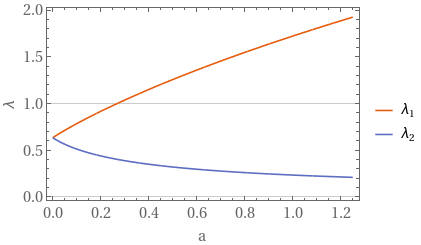
\includegraphics[scale=0.3]{img/EigenP1}
	\caption{Punto fijo 1.}
	\end{subfigure}%
	\begin{subfigure}{.5\textwidth}
	\centering
	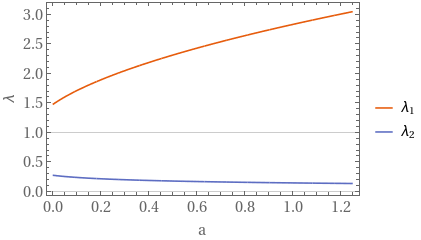
\includegraphics[scale=0.3]{img/EigenP2}
	\caption{Punto fijo 2.}
	\end{subfigure}
	\caption{Eigenvalores.}
	\end{figure}
  \end{itemize}
\end{frame}

%-----------------------------------------------------------------------------
\begin{frame}{Ejemplo: Mapa de Hen�n}
  \begin{itemize}
  \item Para puntos peri�dicos de periodo $2$ se eval�a el Jacobiano $D \vec{f^2}(\vec{p}) = D \vec{f}(\vec{f}(\vec{p})) \cdot D \vec{f}(\vec{p})$.
  \item Este proceso se generaliza para puntos peri�dicos de periodo $n$, evaluando $D \vec{f^{(n)}}(\vec{p})$.
  \item Sea $\vec{p_r}$ un punto de la �rbita peri�dica originada a partir de un punto peri�dico $\vec{p_k}$, entonces
  \[
  	D \vec{f^{(k)}}(\vec{p_r}) = D \vec{f}(p_{r-1}) \cdot D \vec{f}(p_{r-2}) \cdots D \vec{f}(p_{1}) \cdot D \vec{f}(p_{k}) \cdots D \vec{f}(p_{r})
  \]
  \end{itemize}
\end{frame}

%-----------------------------------------------------------------------------
\begin{frame}{Mapa de Hen�n: Puntos fijos}
  \begin{itemize}
  \item Resolviendo $(x,y) = (a-x^2 +by, x)$ se pueden encontrar los puntos fijos. Esta ecuaci�n se reduce a
  \[
  	x^2 + (1-b)x-a=0,
  \]
  cuya soluci�n es
  \[
  	  x = \frac{-(1-b) \pm \sqrt{(1-b)^2 + 4a}}{2}.
  \]
  La condici�n para que esta soluci�n sea real es $4a > -(1-b)^2$.
  \item Esto significa que si $b=0.4$ entonces para que exista un punto fijo $a > -0.09$.
  \end{itemize}
\end{frame}

%-----------------------------------------------------------------------------
\begin{frame}{Mapa de Hen�n: Puntos fijos}
  \begin{itemize}
  \item Para los puntos peri�dicos de periodo 2, se resuelve $(x,y) = f^{(2)}(x,y) = (a-(a-x^2 + by)^2 +bx, a-x^2+by)$.
  \item Desarrollando se llega a
  \[
  	a(1-b)^2-(x^2-a)^2+x(1-b)^3 = 0,
  \]
  cuyas soluciones son
  \[
  	x = \frac{1}{2} \left(b-1 \pm \sqrt{4 a-3 b^2+6 b-3}\right),
  \]
  \[
  	x = \frac{1}{2} \left(1-b \pm \sqrt{4 a+b^2-2 b+1}\right),
  \]
  y la condici�n para que la soluci�n sea real es
  \[
  	4a+6b-3b^2-3 > 0, \quad \rightarrow 4a > 3(b-1)^2.
  \]
  \item Si $b=0.4$, entonces para que exista un punto de periodo 2, $a > 0.27$.
  \end{itemize}
\end{frame}

%-----------------------------------------------------------------------------
\begin{frame}{Mapa de Hen�n: Puntos fijos}
  Todo esto se puede visualizar mejor en un diagrama de bifurcaci�n.
  \begin{figure}[h!]
  	\begin{subfigure}{.5\textwidth}
	\centering
	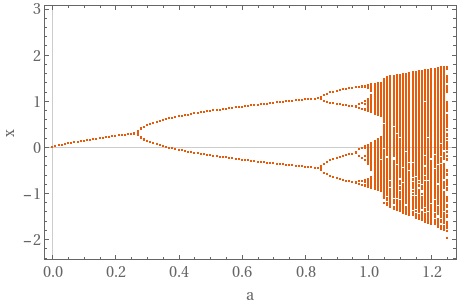
\includegraphics[scale=0.3]{img/HenonBifXA}
	\caption{Variando $a$ con $b=0.4$.}
	\end{subfigure}%
	\begin{subfigure}{.5\textwidth}
	\centering
	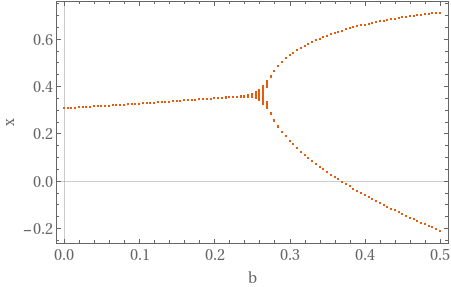
\includegraphics[scale=0.3]{img/HenonBifXB}
	\caption{Variando $b$ con $a=0.4$.}
	\end{subfigure}
	\caption{Diagramas de bifurcaci�n del mapa de Hen�n.}
	\end{figure}
\end{frame}


\end{document}
